\documentclass[12pt]{report}
\usepackage[utf8x]{inputenc}
\usepackage{graphicx}
\usepackage{gensymb}
\usepackage{algorithm}
\usepackage[noend]{algpseudocode}
\usepackage{algpseudocode}
\graphicspath{ {./images/} }
\usepackage{fancyhdr}
\newcommand{\R}{\mathbb{R}}

\title{ETERNITY : FUNCTIONS}								
\author{Juhi Birju Patel}						
\date{23 July 2022}

\makeatletter
\let\thetitle\@title
\let\theauthor\@author
\let\thedate\@date
\makeatother

\pagestyle{fancy}
\fancyhf{}
\rhead{\thetitle}
\cfoot{\thepage}

\begin{document}

\begin{titlepage}
	\centering
    \vspace*{0.5 cm}
\begin{center}    \textbf{\Large Concordia University}\\[2.0 cm]	\end{center}
	\textsc{\Large  SOEN 6011 - Software Engineering Process }\\[0.5 cm]
	\rule{\linewidth}{0.2 mm} \\[0.4 cm]
	{ \huge \textbf \thetitle}\\[0.2 cm]
	{ \huge \textbf{ Function 6 : B(x,y)}}
	\rule{\linewidth}{0.2 mm} \\[1.5 cm]

\begin{center}   {\Large Problem Solution 4}\\[2.0 cm]
\end{center}	
\begin{center}   {\Large \textbf{\theauthor}} \\[0.2 cm]
                 {\large Student ID : 40190446 }\\[0.2 cm]
                 {\large https://github.com/JuhiCodes/SOEN-6011-Course-Project}
\end{center}
	
\end{titlepage}

\tableofcontents
\pagebreak
\renewcommand{\thesection}{\arabic{section}}
\newpage
\section{Debugger - Eclipse}
Debugging for the code is performed using eclipse debugger. Several breakpoints are investigated.
\begin{center}
   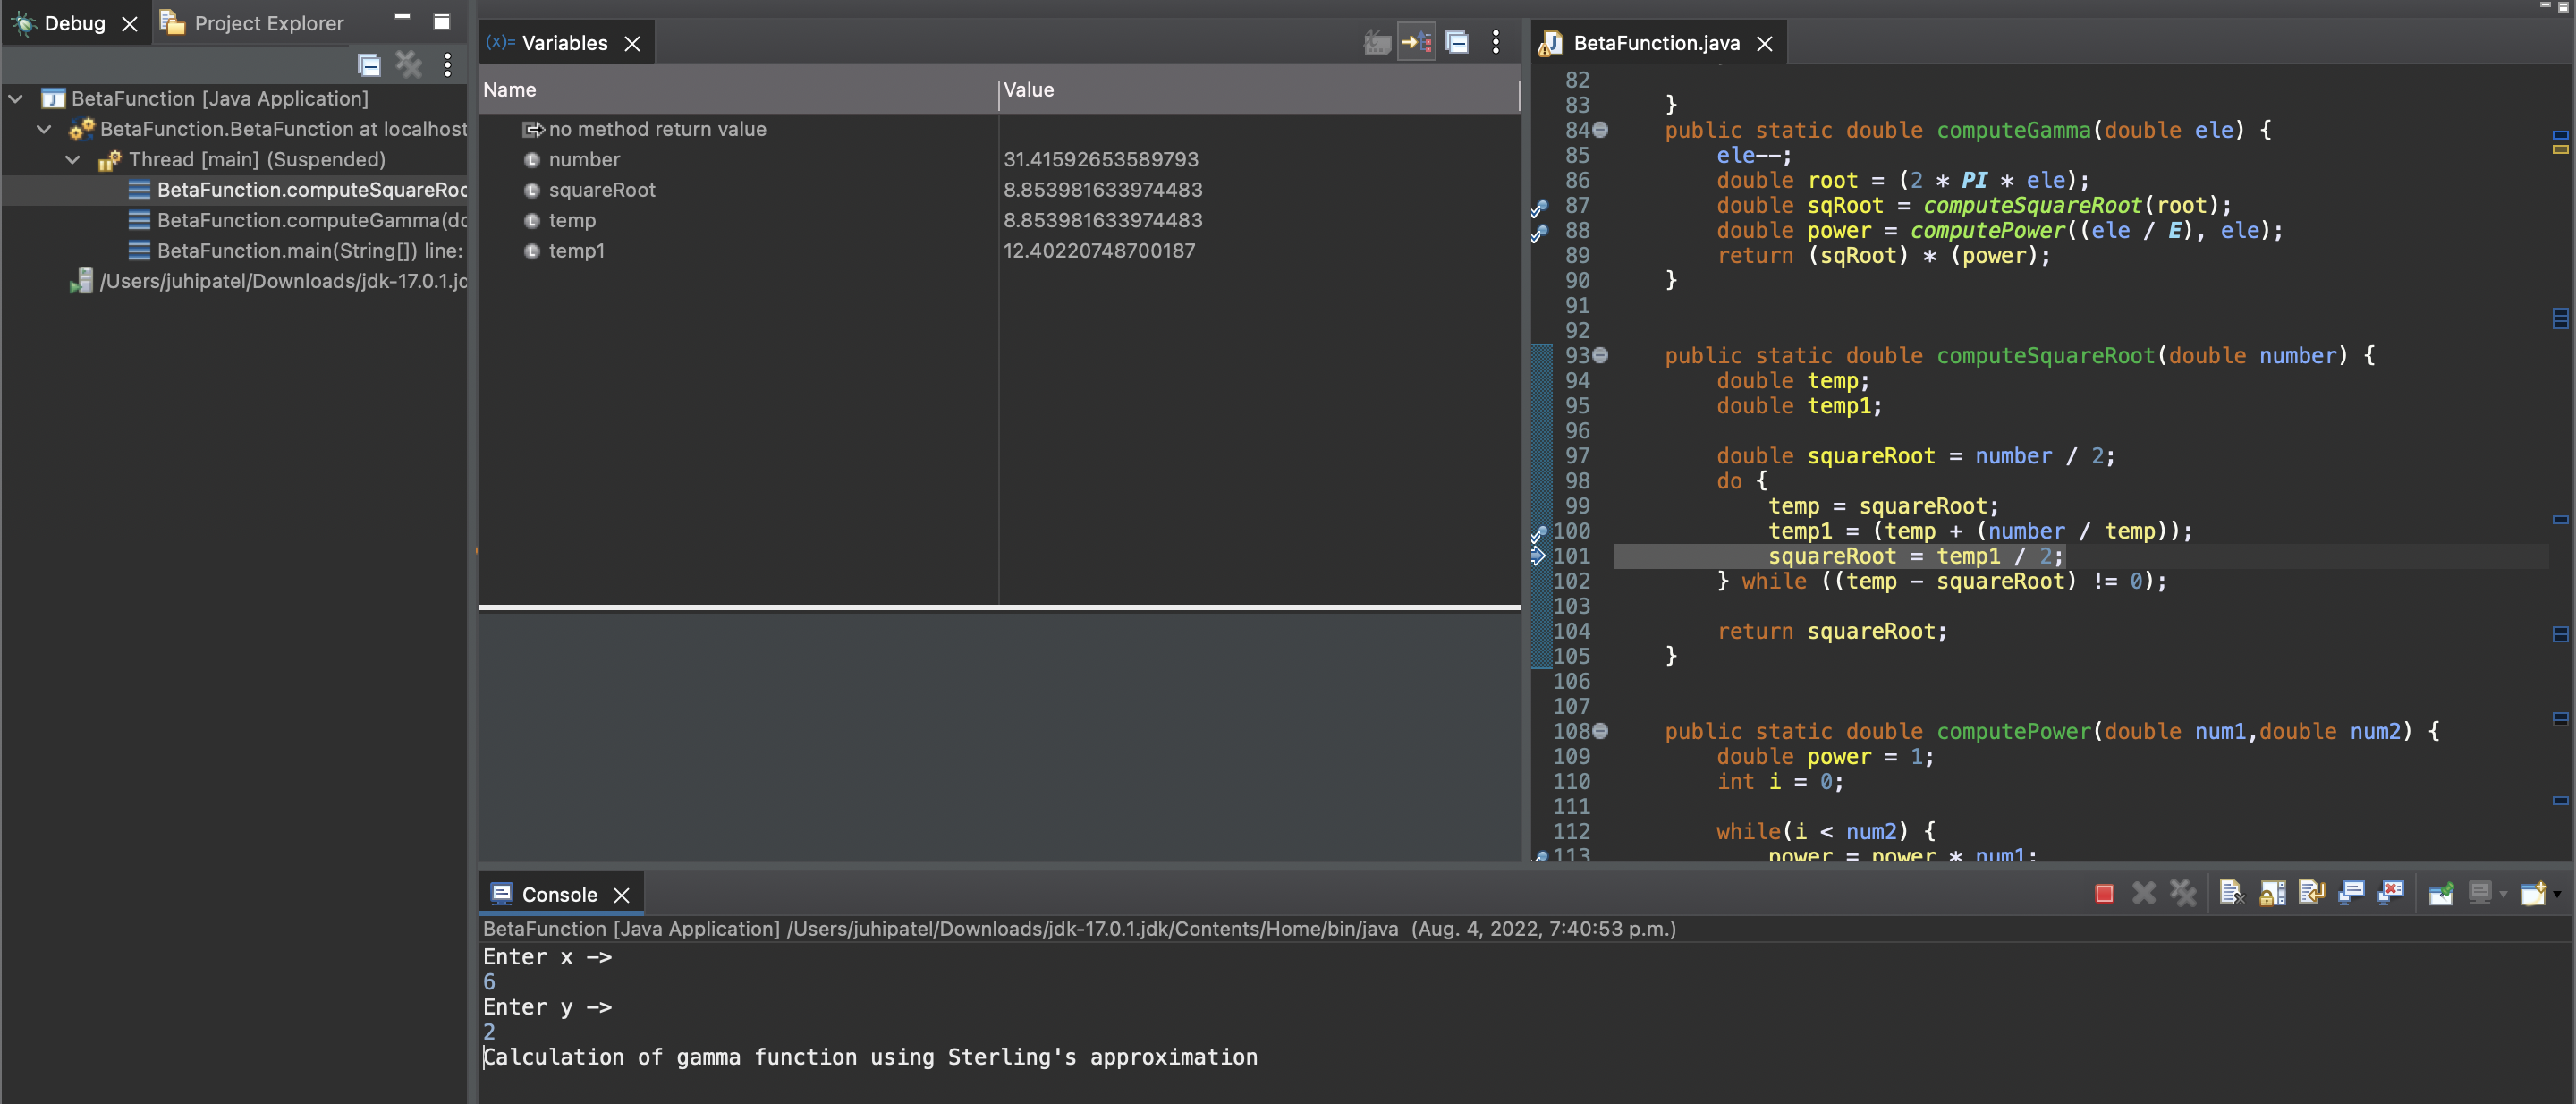
\includegraphics[scale=0.25]{images/eclipse_debugger.png}
\end{center}
    
The Eclipse Java IDE has many debugging tools and views present in the Debug Perspective to help the developer debug the code effectively and efficiently.
A developer can run an application in Debug mode and can iterate over each line of code in a program. In addition to this, Eclipse has a Debug Perspective which is a set of views grouped together that can be helpful to inspect code and make the debugging process very effective.

\subsubsection{Advantages}
\begin{itemize}
\item Eclipse allows you to many event based breakpoints.
\item It provides with filtering options like step into, step over etc.
\item The values of the variables under inspection can be changed while debugging.
\item Developer can view a logical structure of their code.
\end{itemize}

\subsubsection{Disadvantages}
\begin{itemize}
\item Debugging when we have multithreaded programs is difficult.
\item When the program is huge, debugging is not effective with the debugger.
\end{itemize}

\section{Quality Attributes}
Below mentioned are the steps taken to ensure the quality of the source code.
\subsubsection{Correctness}
To check for the correctness of the code, all the input values are validated. The results are compared to the results received from a scientific calculator.
\subsubsection{Robust}
Error handling is used to validate proper inputs. In addition to this, unit testing is performed on the code.
\subsubsection{Time Efficient}
The big O complexity of the code is quite low which makes the code run faster.
\subsubsection{Usable}
The interface is easy to use. Proper messages are displayed on events of taking user inputs and display of error messages. The results are also formatted properly which makes it easy for the user to interpret them.

\section{Source Code review Checkstyle}
Checkstyle is a development tool that aims at helping developers to write Java code that follows a coding standard. It automates the process of checking Java code. 
\begin{center}
   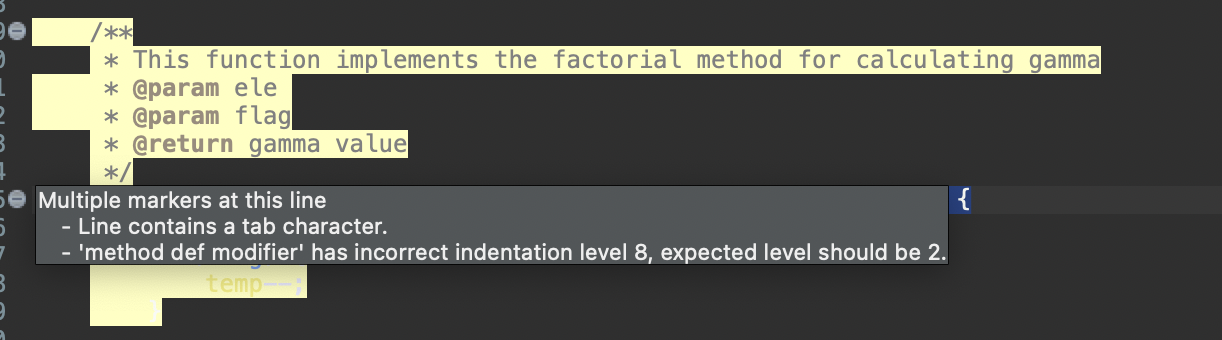
\includegraphics[scale=0.50]{images/checkstyle.png}
\end{center}
The following issues were observed:
\begin{itemize}
\item Most of the error were indentation errors, which were fixed.
\item JavaDoc comments were missing which were added.
\item Else statements were to be added with every if statement.
\item Variable naming did not follow standard naming practice, which was corrected.
\end{itemize}

\newpage
\begin{thebibliography}{9}

\bibitem{wiki}
Eclipse Debugger,
\\\texttt{https://www.eclipse.org/community/eclipse_newsletter/2017/june/article1.php}

\bibitem{checkstyle}
Checkstyle,
\\\texttt{https://checkstyle.sourceforge.io}


\end{thebibliography}
\end{document}
